\section{Cours 10}\label{cours-10}

\subsection{La mémoire}\label{la-muxe9moire}

Accéder à la mémoire directement n'est pas une bonne solution car on
doit connaitre son organisation à la compilation. Impossible car si on
passe de 2 Go de RAM à 4 il faut tout recompiler !! On va virtualiser
tout ça

\subsubsection{La Mémoire Virtuelle}\label{la-muxe9moire-virtuelle}

On va devoir faire une traduction du virtuelle à physique via le
\textbf{MMU} ou \textbf{Memory Management Unit} (qui est dans le
processeur).

\begin{figure}
\centering
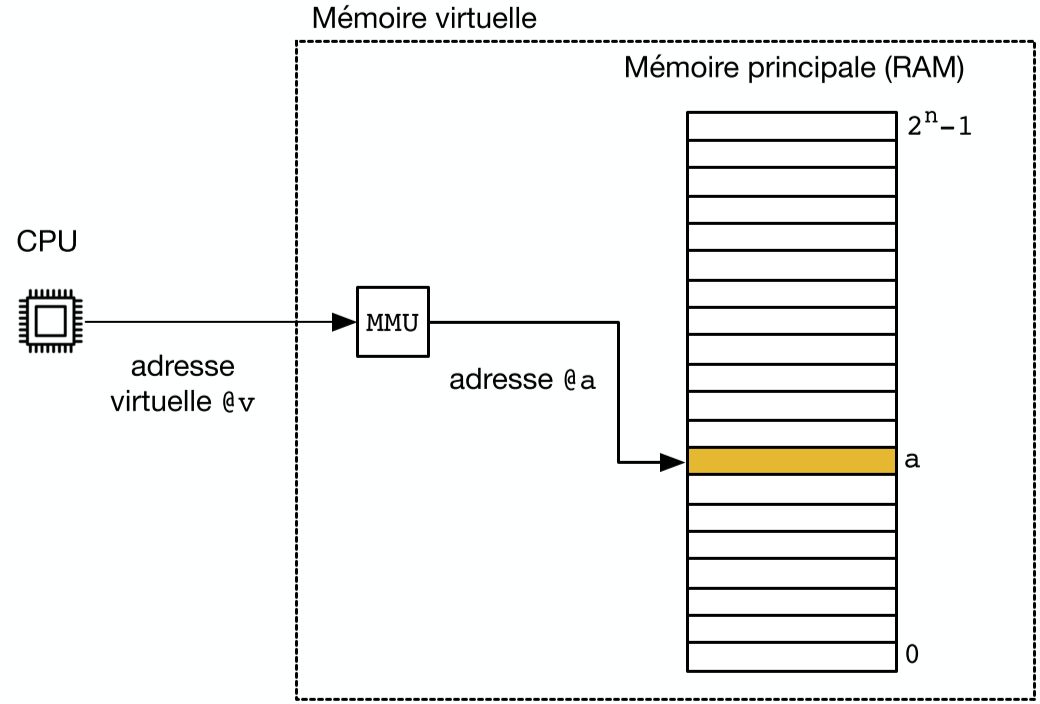
\includegraphics{image-52.png}
\caption{MMU Simple}
\end{figure}

Ainsi on peut découpler la taille et écrire les adresses sur + de 32
bits.

On peut faire de la librairie partagée très facilement, on peut voir que
2 programmes pointes vers la même zone de la RAM !

\paragraph{Avantages}\label{avantages}

On peut utiliser le stockage sur le disque pour mettre des objets
inutilisées de la RAM. C'est le principe de \textbf{\texttt{swap}}. Et
on peut faire vice-versa.

\subsubsection{Fonctionnement de la mémoire
Virtuelle}\label{fonctionnement-de-la-muxe9moire-virtuelle}

La mémoire a un accès par \emph{adresse} et les SSD par \emph{secteur}.
La mémoire virtuelle est divisée par \textbf{pages}. C'est une zone de
mémoire \textbf{contiguë} de taille 4 Ko (4096 octets (on peut vérifier
via \texttt{getpagesize()})).

On a toujours un nombre entier de pages. De plus, chaque segment (les 6)
occupe leurs propres pages.

Ainsi, les pages virtuelles peuvent être placées dans n'importe quelle
zone (\emph{frame}/cadre de page) de la mémoire physique.

Adresse Virtuelle est composée de:

\begin{itemize}
\tightlist
\item
  Numéro de la page
\item
  Offset sur cette page à faire
\end{itemize}

Le MMU se charge de la traduction.

\begin{figure}
\centering
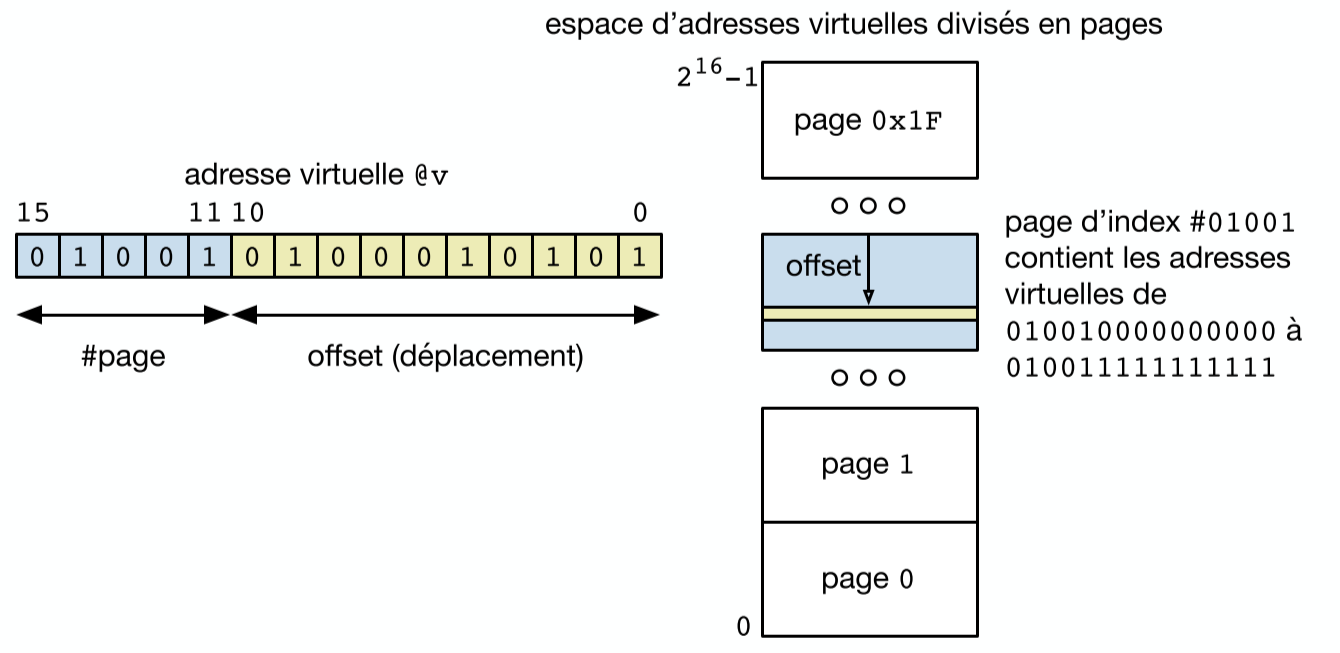
\includegraphics{image-53.png}
\caption{Découpage en page}
\end{figure}

\subsubsection{Mise en Oeuvre de la
Traduction}\label{mise-en-oeuvre-de-la-traduction}

Il doit avoir accès à l'allocation actuelle entre pages virtuelles et
cadres de pages physique. On va utiliser une table des pages:

\begin{itemize}
\tightlist
\item
  Tableau indexé par le numéro de page
\item
  Bit de validité si la page existe dans l'espace mémoire du
  \emph{processus}
\item
  Si valide: ligne du tableau indique le lien vers le numéro de cadre de
  page.
\end{itemize}

\begin{figure}
\centering
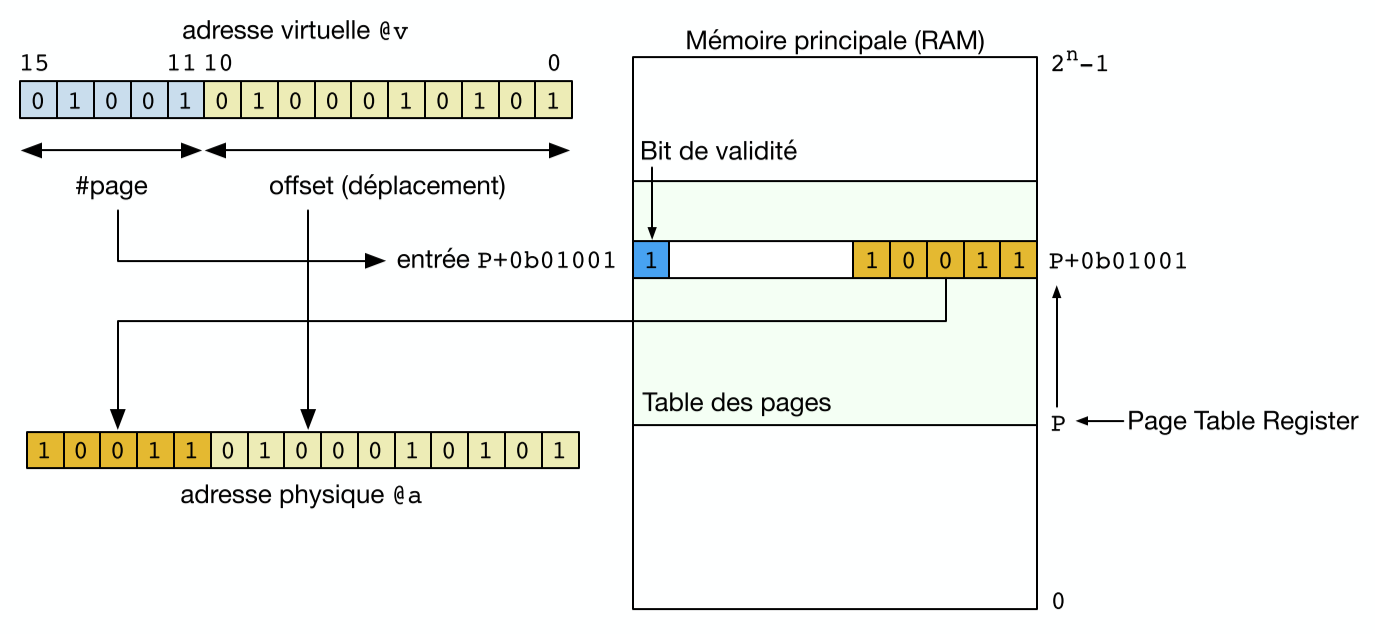
\includegraphics{image-54.png}
\caption{Traduction}
\end{figure}

Chaque processus possède donc sa \textbf{propre table des pages} (pas
pour le kernel). On a un registre spécial qui contient l'adresse de base
en mémoire de la table des pages du processus actuel (restauré à chaque
rétablissement de contexte).

\paragraph{Exemple pour 2 processus}\label{exemple-pour-2-processus}

Si on a un système 8 bits (RAM maximum de 256) ce qui nous donne 16
cadres de pages de 16 octets chacun. On décide d'avoir des adresses
virtuelles sur 6 bits donc un maximum de 64 octets par processus (chaque
processus va donc utiliser 4 pages --\textgreater{} 2 bits pour la page
4 pour l'offset).

Imaginons 2 processus \texttt{P1} et \texttt{P2} qui requiert 3 pages (2
pour leur text et 1 pour leur stack).

\begin{figure}
\centering
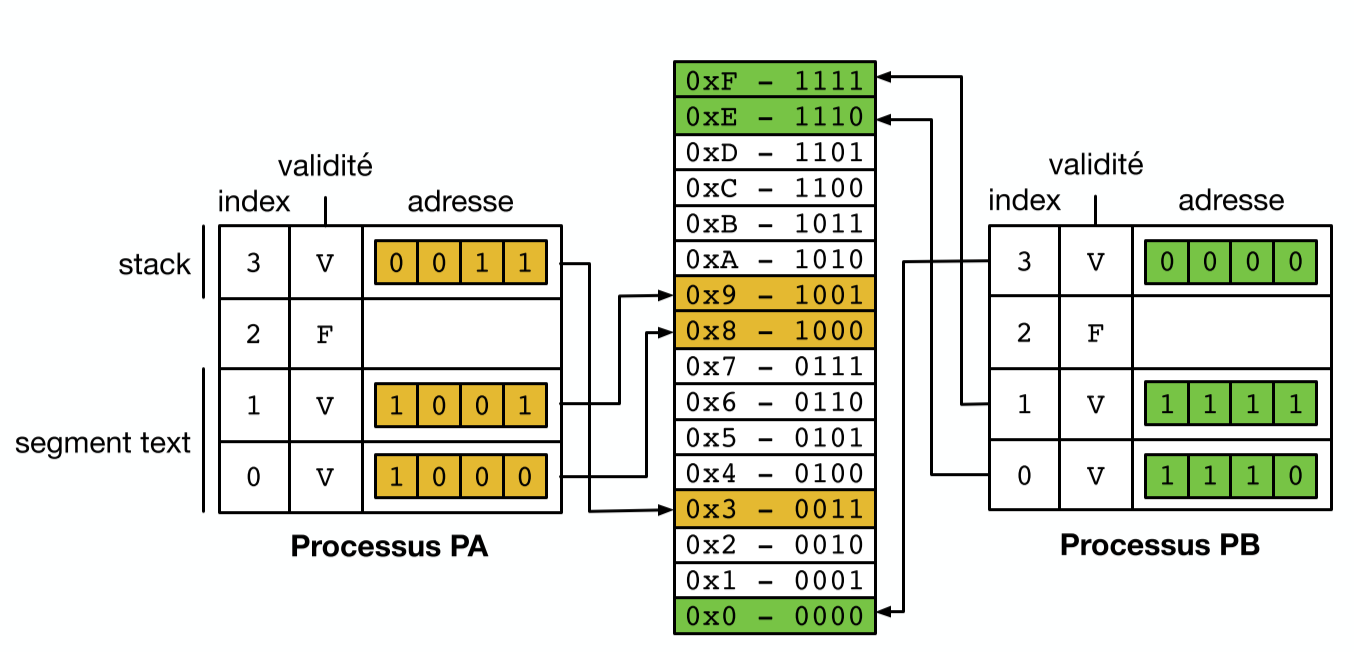
\includegraphics{image-55.png}
\caption{Exemple P1 et P2}
\end{figure}

On remarque que faire la traduction entre adresse physique et virtuelle
requiert 1 accès en plus. On va donc mettre en \emph{cache} les
traductions souvent utilisées via un \textbf{TLB} ou \textbf{Translation
Lookaside Buffer} ce qui nous donne un fonctionnement de la sorte.

\begin{figure}
\centering
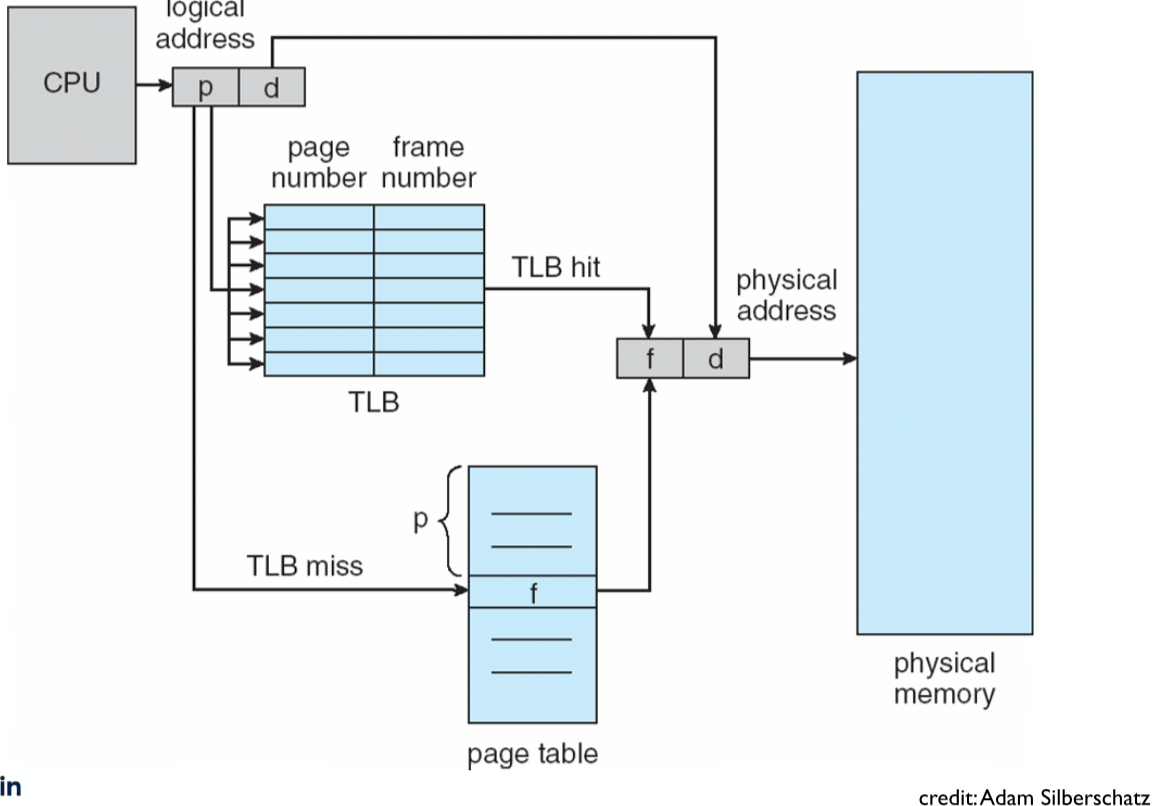
\includegraphics{image-56.png}
\caption{TLB hit et miss}
\end{figure}

\subsubsection{Protection des Pages}\label{protection-des-pages}

On peut encoder les droits d'une page sur 3 bits: \texttt{R}, \texttt{W}
et \texttt{X}. Si on essaye de faire une action invalide, on génère
ainsi un trap qui passe la main au SE. Sous Linux, on a une page par
processeur.

On peut retirer des droits à une page via:

\begin{Shaded}
\begin{Highlighting}[]
\PreprocessorTok{\#include }\ImportTok{\textless{}sys/mman.h\textgreater{}}\PreprocessorTok{ }

\DataTypeTok{int}\NormalTok{ mprotect}\OperatorTok{(}\DataTypeTok{const} \DataTypeTok{void} \OperatorTok{*}\NormalTok{addr}\OperatorTok{,} \DataTypeTok{size\_t}\NormalTok{ len}\OperatorTok{,} \DataTypeTok{int}\NormalTok{ prot}\OperatorTok{);}
\end{Highlighting}
\end{Shaded}

\subsubsection{Problème du Swap}\label{probluxe8me-du-swap}

On a 2 façon de faire du swap (qui permet d'avoir plus de pages
virtuelles):

\begin{enumerate}
\def\labelenumi{\arabic{enumi}.}
\tightlist
\item
  Partition de Swap:

  \begin{itemize}
  \tightlist
  \item
    ✅ Rapide
  \item
    ❌ Portion du disque dédiée
  \end{itemize}
\item
  Fichier de Swap:

  \begin{itemize}
  \tightlist
  \item
    ✅ Flexible
  \item
    ❌ Performance moindre (fragmentation du fichier)
  \end{itemize}
\end{enumerate}

\paragraph{Fonctionnement par défaut d'un accès à une
page}\label{fonctionnement-par-duxe9faut-dun-accuxe8s-uxe0-une-page}

\begin{figure}
\centering
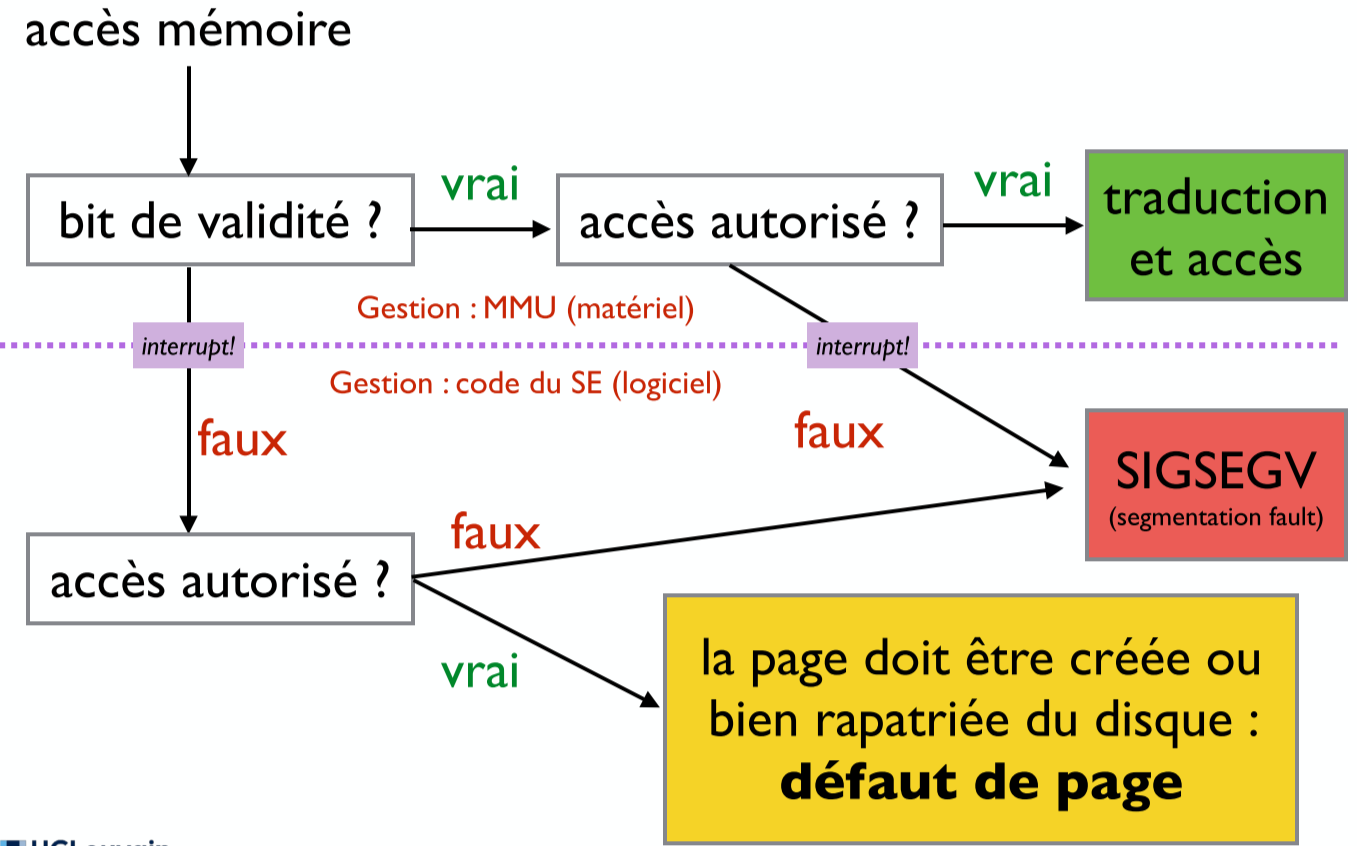
\includegraphics{image-57.png}
\caption{Défauts de page}
\end{figure}

\begin{figure}
\centering
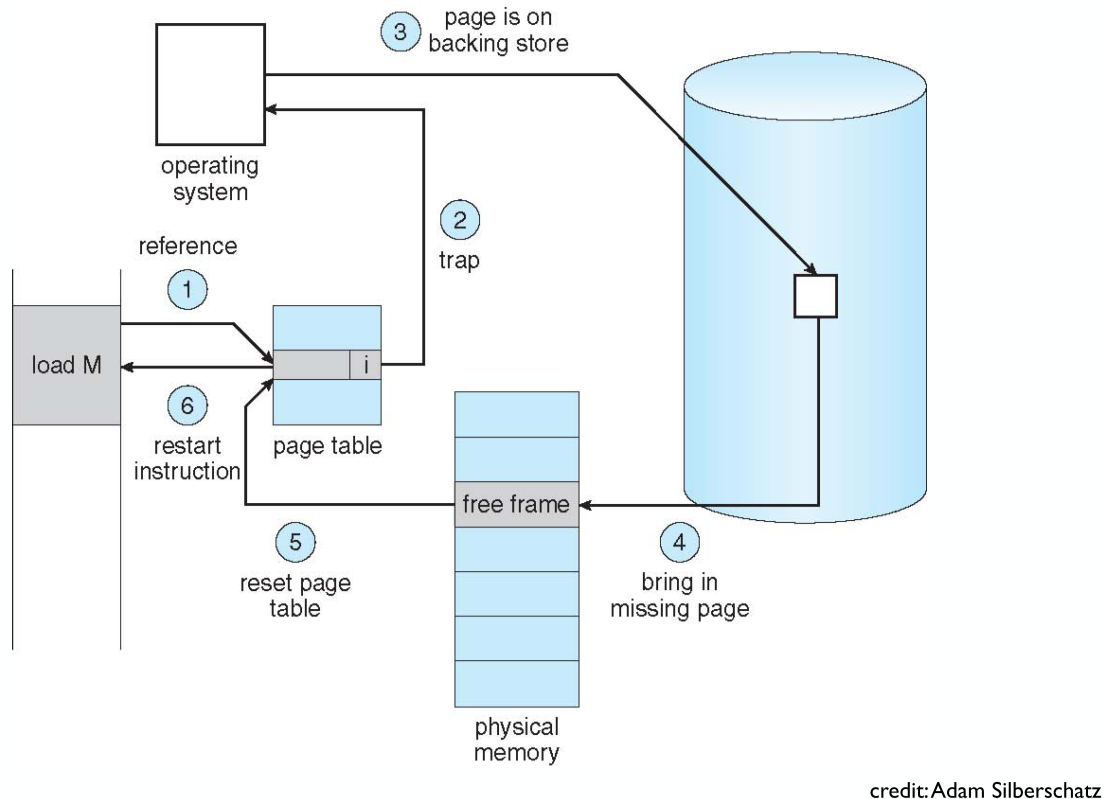
\includegraphics{image-58.png}
\caption{Traitement d'un défaut de page}
\end{figure}

On va donc devoir rapatrier des pages du disque vers la mémoire si on
constate un défaut de page (ou en créer une nouvelle).

On va devoir aussi faire une politique de suppression des pages les plus
anciennes et des moins utilisées. Cela va suivre des critères bien
précis:

\begin{itemize}
\tightlist
\item
  Métadonnées qui ne rajoutent pas de la lourdeur (utilisée des bits des
  pages non utilisés)
\item
  Ne pas supprimer des pages qui sont souvent utiliser ou va l'être.
\end{itemize}

On va \textbf{éviter} ces 2 politiques:

\begin{enumerate}
\def\labelenumi{\arabic{enumi}.}
\tightlist
\item
  FIFO: supprimer les pages les plus anciennes. Ne prend pas en compte
  le fait qu'on utilise activement une page
\item
  Conserver des statistiques sur les accès: irréalistes et coûteux.
\end{enumerate}

On va utiliser le principe du \textbf{LRU} ou \textbf{Least Recently
Used} pour enlever la page utilisée en dernier. On va faire cela sans
compter le temps. On va tous les X cycles d'horloges checker 2 bits
spécifiques:

\begin{enumerate}
\def\labelenumi{\arabic{enumi}.}
\tightlist
\item
  Dirty bit: page modifiée ? \emph{page modifiée et à mettre à jour sur
  le disque}
\item
  Reference bit: page utilisée ? \emph{page accédée récemment}
\end{enumerate}

\begin{figure}
\centering
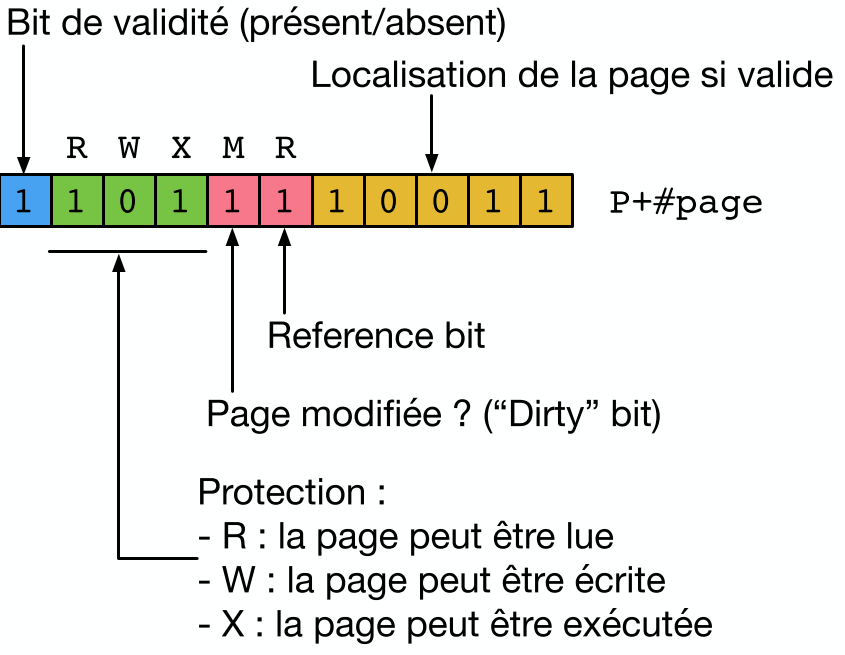
\includegraphics{image-60.png}
\caption{Format complet d'une entrée de la table des pages}
\end{figure}

Après chaque check, le SE va mettre ces 2 bits à 0. On va supprimer en
premier les pages qui sont \texttt{00} et \texttt{01} car elles ne sont
pas accédées.

\subsubsection{Fichiers Mappés en
Mémoire}\label{fichiers-mappuxe9s-en-muxe9moire}

On peut mapper le contenu d'un fichier dans la mémoire pour avoir plus
simple à le manipuler (👀 oui
\href{https://media.discordapp.net/attachments/517720163223601155/1113851521029910569/GOODBOOOOOI.gif}{@Hokkaydo})
via cet appel système qui nous renvoie un pointeur vers la zone mappée
ou un \texttt{MAP\_FAILED}:

\begin{Shaded}
\begin{Highlighting}[]
\PreprocessorTok{\#include }\ImportTok{\textless{}sys/mman.h\textgreater{}}\PreprocessorTok{ }

\DataTypeTok{void} \OperatorTok{*}\NormalTok{mmap}\OperatorTok{(}\DataTypeTok{void} \OperatorTok{*}\NormalTok{addr}\OperatorTok{,} \DataTypeTok{size\_t}\NormalTok{ length}\OperatorTok{,} \DataTypeTok{int}\NormalTok{ prot}\OperatorTok{,} \DataTypeTok{int}\NormalTok{ flags}\OperatorTok{,} \DataTypeTok{int}\NormalTok{ fd}\OperatorTok{,}\NormalTok{ off\_t offset}\OperatorTok{);}
\CommentTok{/*}
\CommentTok{* addr:     où on veut mapper, Généralement NULL}
\CommentTok{* length:   longueur de la zone du fichier à mapper}
\CommentTok{* prot:     permission (R/W/X)}
\CommentTok{* flags:    mapping privé (MAP\_PRIVATE) ou partagé entre processus (MAP\_SHARED)}
\CommentTok{* fs:       descripteur du fichier}
\CommentTok{* offset:   où on veut démarrer à mapper}
\CommentTok{*/}
\end{Highlighting}
\end{Shaded}

\begin{figure}
\centering
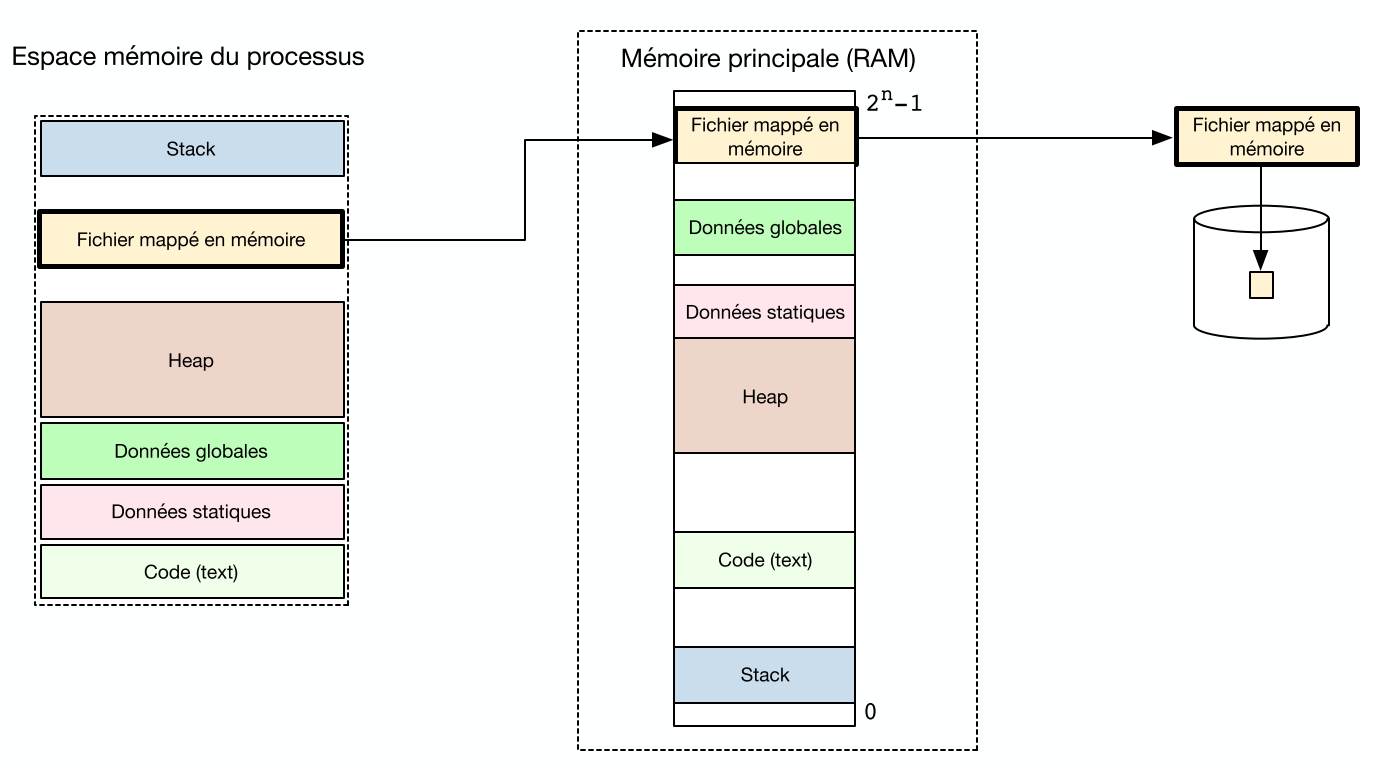
\includegraphics{image-61.png}
\caption{Mapping en Mémoire}
\end{figure}

\paragraph{Appels Systèmes
Associés}\label{appels-systuxe8mes-associuxe9s}

On peut forcer l'écriture sur le disque (même idée de buffer que pour
\texttt{printf}):

\begin{Shaded}
\begin{Highlighting}[]
\PreprocessorTok{\#include }\ImportTok{\textless{}sys/mman.h\textgreater{}}\PreprocessorTok{ }

\DataTypeTok{int}\NormalTok{ msync}\OperatorTok{(}\DataTypeTok{void} \OperatorTok{*}\NormalTok{addr}\OperatorTok{,} \DataTypeTok{size\_t}\NormalTok{ length}\OperatorTok{,} \DataTypeTok{int}\NormalTok{ flags}\OperatorTok{);}
\end{Highlighting}
\end{Shaded}

Supprimer tout le mapping ou une partie

\begin{Shaded}
\begin{Highlighting}[]
\PreprocessorTok{\#include }\ImportTok{\textless{}sys/mman.h\textgreater{}}\PreprocessorTok{ }

\DataTypeTok{int}\NormalTok{ munmap}\OperatorTok{(}\DataTypeTok{void} \OperatorTok{*}\NormalTok{addr}\OperatorTok{,} \DataTypeTok{size\_t}\NormalTok{ length}\OperatorTok{);}
\end{Highlighting}
\end{Shaded}

\subsubsection{Mémoire partagée}\label{muxe9moire-partaguxe9e}

Quand on a plusieurs threads, la table des pages est copiée pour tous
les segments \textbf{sauf le Stack}.

On peut faire de la communication entre processus via de la mémoire
partagée. Il faut que les entrées de la table des pages des deux
processus pointent vers les mêmes frames physiques.

\paragraph{Gestion de la mémoire
partagée}\label{gestion-de-la-muxe9moire-partaguxe9e}

\begin{longtable}[]{@{}
  >{\centering\arraybackslash}p{(\columnwidth - 4\tabcolsep) * \real{0.2478}}
  >{\centering\arraybackslash}p{(\columnwidth - 4\tabcolsep) * \real{0.4696}}
  >{\centering\arraybackslash}p{(\columnwidth - 4\tabcolsep) * \real{0.2826}}@{}}
\toprule\noalign{}
\begin{minipage}[b]{\linewidth}\centering
Fonction
\end{minipage} & \begin{minipage}[b]{\linewidth}\centering
Paramètre
\end{minipage} & \begin{minipage}[b]{\linewidth}\centering
Description
\end{minipage} \\
\midrule\noalign{}
\endhead
\bottomrule\noalign{}
\endlastfoot
\texttt{int\ shmget(key\_t,\ key,\ size\_t\ size,\ int\ shmflg)} &
\texttt{key}: une clé. \texttt{size}: taille de page. \texttt{shmflg}:
on le met à \texttt{IPC\_CREAT} pour créer sinon obtenir un accès. &
crée ou obtient l'accès à un segment de mémoire partagée \\
\texttt{void\ *shmat(int\ shmid,\ const\ void\ *shmaddr,\ int\ shmflg)}
& \texttt{shmid}: id de la page qu'on a obtenu. \texttt{shmaddr}: mis à
\texttt{NULL}. \texttt{shmflg}: mis à 0. & Pour attacher la page
partagée dans l'espace mémoire du processus \\
\texttt{int\ shmdt(const\ void\ *shmaddr)} & \texttt{shmaddr}: l'adresse
retournée par \texttt{shmat}. & Pour détacher la page \\
\end{longtable}

\texttt{shmget} va pousser le kernel à mettre toutes les valeurs à 0
dans l'ensemble des adresses concernées pour des raisons de sécurité.

Il faut faire attention à ce que la mémoire soit bien attachée pour les
deux processus. On va soit:

\begin{enumerate}
\def\labelenumi{\arabic{enumi}.}
\tightlist
\item
  éviter d'utiliser des pointeurs (sinon il ne pointe pas vers les mêmes
  choses dans le processus)
\item
  stocker les adresses relatives au début de la zone mémoire partagée
\end{enumerate}

\paragraph{Destruction des segments
partagés}\label{destruction-des-segments-partaguxe9s}

Les segments partagées vont continuer à exister même à la terminaison du
processus créateur. On utilise \texttt{shmctl} pour supprimer un
segment. La suppression se fera au dernier \texttt{shmdt}.

\paragraph{Librairie partagée}\label{librairie-partaguxe9e}

La zone mémoire liée aux librairies partagées se trouvent entre le stack
et le heap et sera en \texttt{.so}.

\begin{figure}
\centering
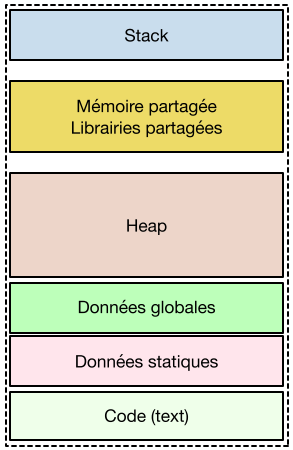
\includegraphics{image-62.png}
\caption{Espace mémoire du processus}
\end{figure}

\subsubsection{\texorpdfstring{Fonctionnement de \texttt{fork} et
\texttt{exec}}{Fonctionnement de fork et exec}}\label{fonctionnement-de-fork-et-exec}

En faisant un \texttt{fork} on va faire une copie de la table des pages
en mode read pour le segment text sinon en mode écriture, il faut
réaliser une isolation le \textbf{Copy-on-Write}.

\paragraph{Copy-on-Write}\label{copy-on-write}

Les pages sont déclarées en \emph{read-only} donc essayer d'écrire va
générer un trap. Le SE va vérifier si l'accès interdit est pour une page
réellement en écriture. Si c'est le cas:

\begin{itemize}
\tightlist
\item
  La page est dupliquée vers une nouvelle page
\item
  Table des pages mise à jour pour pointer vers cette copie
\item
  On redémarre l'instruction qui a générée l'erreur
\end{itemize}

\begin{figure}
\centering
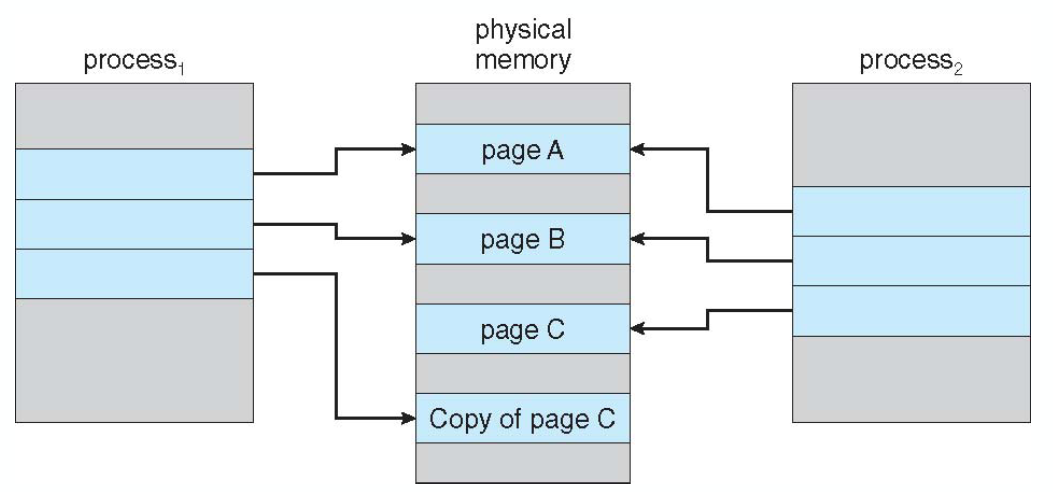
\includegraphics{image-63.png}
\caption{Copy-on-Write: après}
\end{figure}
